\documentclass[../mainfile.tex]{article}
% Kopiert von kurbaniec :) 

\begin{document}
\section{Konvergenz / Divergenz}
\subsection{Definition:}

Eine Folge $a_{n}$ heißt konvergent, falls eine Zahl $a$ existiert, soo dass die folgende Bedingung erfüllt ist:\\
Zu jedem $\epsilon > 0$ existiert ein $N \in \mathbb{N}$, so dass ab diesem Folgeglied alle Folgeglieder innerhalb der $\epsilon$-Umgebung um $a$ liegen.\\
\quad\\
D.h. $\forall \epsilon > 0 \exists N \in \mathbb{N} \forall n > N: |a_{n}-a| < \epsilon$\\
\quad\\
$a$ heißt Grenzwert von $a_{n}$\\
Schreibweise: $\lim\limits_{n \rightarrow \infty}{a_{n}} = a$\\
Ist $a_{n}$ nicht konvergent, dann heißt $a_{n}$ divergent.

\subsection{Erklärung:}
\FloatBarrier
\begin{figure}[!htbp] 
\centering
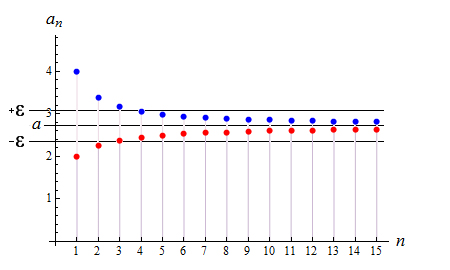
\includegraphics[width=8cm]{./swahl/img/konvergenzGraph.jpg}
\caption{Darstellung anhand eines Graphen}
\end{figure}
\FloatBarrier

Wichtigster Grenzwert:\\
$\lim\limits_{n \rightarrow \infty}{\frac{1}{n}} = 0$\\
\quad\\
Wie viele Grenzwerte kann eine Folge besitzen? $\Rightarrow$ Es kann nur einen Grenzwert geben! 
	
\end{document}